\documentclass[10pt,a4paper]{article}

\usepackage[utf8]{inputenc}
\usepackage[T1]{fontenc}
\usepackage[french,english]{babel}
\usepackage{blindtext}

\usepackage[hyphens]{url}
\usepackage{hyperref}
\DeclareUrlCommand\email{\urlstyle{rm}}

\usepackage[margin=2in]{geometry} % showframe
\usepackage{multicol}

\usepackage{graphicx}
\usepackage{xcolor}
\usepackage{amsmath}
\usepackage{amsthm}
\usepackage{amsfonts}
\usepackage{amssymb}
\usepackage{siunitx}
\usepackage{pdflscape}
%\usepackage[toc]{glossaries} % https://www.overleaf.com/learn/latex/Glossaries
%\usepackage{parskip} % empty line between paragraphs
\usepackage{listings}
\usepackage{float}
\usepackage{pmboxdraw}
\usepackage{textcomp} % for the apostrophe
\usepackage{float}
\usepackage{comment}

% hyperref setup
\definecolor{darkgreen}{RGB}{0,180,0}
\hypersetup{
    colorlinks = true,
    linkbordercolor = {white},
    linkcolor = red,
    anchorcolor = black,
    citecolor = darkgreen,
    filecolor = cyan,
    menucolor = black,
    runcolor = cyan,
    urlcolor = magenta
}

% Bib setup
\usepackage{csquotes} % Recommended by biblatex
\usepackage[style=numeric,sorting=none,backend=biber]{biblatex}
\DeclareBibliographyAlias{software}{online}
\addbibresource{references.bib} % The file containing our references, in BibTeX format


\newcommand{\htriple}[3]{\ensuremath{\{#1\}~#2~\{#3\}}}
\newcommand{\WP}{\ensuremath{\mathit{WP}}}
\newcommand{\notimplies}{%
  \mathrel{{\ooalign{\hidewidth$\not\phantom{=}$\hidewidth\cr$\implies$}}}}
\newcommand{\eqdef}{\stackrel{def}{=}}
\newcommand{\eqeval}{\stackrel{eval}{=}}

\newtheorem{theorem}{Theorem}[section]
\newtheorem{corollary}{Corollary}[theorem]
\newtheorem{lemma}[theorem]{Lemma}
\newtheorem{remark}{Remark}
\newtheorem*{remark*}{Remark}

%% Listing settings
\definecolor{codegreen}{rgb}{0,0.6,0}
\definecolor{codegray}{rgb}{0.5,0.5,0.5}
\definecolor{codepurple}{rgb}{0.58,0,0.82}
\definecolor{codeblue}{rgb}{0.10,0,0.82}
\definecolor{codebackcolour}{rgb}{0.95,0.95,0.92}
 


\title{Experiments on automation of formal verification of devices at the binary level}
\author{Thomas Lacroix --- \email{thomas.lacroix@insa-lyon.fr}\medskip\\
Département Informatique\\
INSA de Lyon}
\date{2018/2019}

\begin{document}

\newgeometry{margin=2cm}

\maketitle
\thispagestyle{empty}

{
\noindent Sous la responsabilité de :\\
\indent Mads Dam : Division of Theoretical Computer Science -- KTH\\
\indent Pierre-\'Edouard Portier : Département Informatique -- INSA Lyon
}

\vspace{\baselineskip}\vspace{\baselineskip}

{ % Block used for font size in abstracts
\fontsize{9}{10.8}

\begin{abstract}
  \rightmargin=1cm \leftmargin=1cm
  With the advent of virtualization, more and more work is put into the verification of hypervisors. Being low-level softwares, such verification should preferably be performed at binary level. Binary analysis platforms are being developed to help perform these proofs, but a lot of the work has to be carried out manually.

  In this thesis, we focus on the formal verification of a Network Interface Controller (NIC), more specifically we look at how to automate and reduce the boilerplate work from an existing proof. We base our work on the HolBA platform, its hardware-independent intermediate representation language BIR and supporting tools, and we experiment on how to perform this proof by leveraging existing tools.

  We first replaced the existing NIC model written in HOL4 to an equivalent one written using BIR, enabling the use of HolBA tools. Secondly, we developed some visualization tools to help navigate and gain some insight into the existing proof and its structure. Thirdly, we experimented with the use of Hoare triples in conjunction with an SMT solver to perform contract verification. Finally, we proved a simple contract written in terms of the formal NIC model on the BIR implementation of this model, unlocking the way of performing more complex proofs using the HolBA platform.
\end{abstract}

\leftmargin=1cm
{\small\textbf{\textit{Keywords---}} binary analysis, formal verification, proof producing analysis, theorem proving}

\vspace{\baselineskip}\vspace{\baselineskip}

\begin{otherlanguage}{french}
  \begin{abstract}
    \rightmargin=1cm \leftmargin=1cm
    Avec la démocratisation de la virtualisation, de plus en plus d'efforts sont consacrés à la vérification des hyperviseurs. S'agissant de logiciels de bas niveau, une telle vérification devrait de préférence être effectuée au niveau binaire. Des plates-formes d'analyse binaire sont en cours de développement pour aider à réaliser ces preuves, mais une grande partie du travail doit encore être effectuée manuellement.

    Dans cette thèse, nous nous concentrons sur la vérification formelle d'un Contrôleur d'Interface Réseau (NIC), plus spécifiquement sur la manière d'automatiser et de réduire le travail répétitif d'une preuve existante. Nous nous basons sur la plate-forme HolBA, son langage de représentation intermédiaire indépendant du matériel, BIR et ses outils de support, et nous nous intéressons à la manière de réaliser cette preuve en utilisant des outils existants.

    Nous avons d'abord remplacé le modèle NIC existant écrit en HOL4 par un modèle équivalent écrit en BIR, permettant ainsi l'utilisation des outils de HolBA. Deuxièmement, nous avons développé des outils de visualisation pour nous aider à naviguer et à mieux comprendre la preuve existante et sa structure. Troisièmement, nous avons expérimenté l'utilisation des triplets de Hoare en conjonction avec un solveur SMT pour effectuer une vérification par contrat. Enfin, nous avons prouvé un contrat simple écrit en termes du modèle formel du NIC sur l'implémentation de ce modèle en BIR, ouvrant la voie à la réalisation de preuves plus complexes avec la plate-forme HolBA.
  \end{abstract}
\end{otherlanguage}

\leftmargin=1cm
{\small\textbf{\textit{Mot-clés---}} binary analysis, formal verification, proof producing analysis, theorem proving}
}

\vspace{\baselineskip}\vspace{\baselineskip}

\restoregeometry
\newgeometry{margin=3cm}
\fontsize{10}{12}\selectfont
%--------------------------

\begin{multicols}{2}

\section{Introduction}
\textit{This section serves as an introduction to the degree project and presents the background of the work along with this thesis objective. Delimitations to the project and the choice of the methodology are also discussed.}

\subsection{Background}

Embedded systems are becoming more and more common with the current advent of {IoT} and mobile computing platforms, such as smartphones. Those systems are fully-fledged computers with powerful hardware, complete operating systems, and access to the Internet. Such systems can run security-critical services, such as a building security system or automatic toll gates, or carry valuable information as it is the case for personal smartphones. Therefore, these two characteristics make them targets of choice for attackers.

The {PROSPER} project \cite{noauthor_prosper:_nodate} aims to develop a secure and formally verified hypervisor for embedded systems. Hypervisors are thin layers running directly on top of hardware providing the ability to run virtualized applications, such that operating systems or real-time control systems. Those virtualized applications then don't have privileged access to the hardware and have to go through the hypervisor. This allows different applications to share the same hardware while providing strong isolation between them, thus ensuring confidentiality and security. Moreover, security not only means protection from external attacks but also resilience to bugs. If multiple critical systems are running on the same hardware, bugs or crashes in some systems shouldn't affect the others from behaving correctly.

Previous work in the {PROSPER} project achieved to formally verify a simple separation kernel \cite{noauthor_prosper:_nodate-1,dam_formal_2013}, which later resulted into an implementation of a working hypervisor. Then, they achieved to run both Linux and {FreeRTOS} on top of it. Finally, they formally verified memory isolation for virtualized applications \cite{nemati_trustworthy_2015}. However, hardware devices were not included in the verification, so devices, like Network Interface Controller ({NIC}), cannot be used by the virtualized applications reducing the value of the hypervisor. In order to solve this issue, verification of hardware devices is being carried out.

A formal model of a {NIC} device has already been produced, on which some security theorems have been proved \cite{haglund_formal_2016}. These theorems can be seen as high-level proofs relying on a layer of lower-level lemmas. This layer provides an abstraction over the raw formal model. This is illustrated in the left-hand side of Figure \ref{hol-v-bir-nic-model-simple}. However, there exist more devices that are of interest to verify, so it is very desirable to automate formal verification of devices and use a standard model for reasoning about them.

\begin{figure}[H]
  \centering
	\includegraphics[height=6cm]{figures/hol-v-bir-nic-model-simple.png}
	\caption{Formal v. BIR NIC models. The left hand side already exists. The dashed elements represent the work done during this project.}
	\label{hol-v-bir-nic-model-simple}
\end{figure}

The team is now developing a new framework for performing binary analysis in HOL4, an interactive theorem prover, named {HolBA} \cite{noauthor_holba_2019}. This framework features a machine-independent Binary Intermediate Representation (BIR), a proof-producing transpiler from ARMv8 and Cortex-M0 assembly code to BIR, called the lifter, a proof-producing weakest precondition generator for loop-free programs, and supporting tools \cite{metere_sound_2017,lindner_trabin:_2019}.

The idea of this work is to translate the formal {NIC} model of \cite{haglund_formal_2016} using {BIR}, then use HolBA's proof-producing weakest precondition tool to prove the same lower-level lemmas than the formal model. With all the lemmas proved, the security properties are implied. Figure \ref{hol-v-bir-nic-model-simple} gives an overview of this idea: using the proof-producing weakest precondition tool to bind together a newly written BIR NIC model and the work done on the formal model.

\subsection{Thesis objective}

The goal of this thesis project is to explore verification techniques in order to automate parts, if not all, of the verification process of hardware devices using the HolBA platform. The formal {NIC} model of \cite{haglund_formal_2016} is used as working example.

\subsection{Delimitations}

This work being about exploration of techniques towards automation of verification techniques, instead of being about producing an actual complete proof of a hardware device, some implementations have not been completed in order to save time to explore in more areas. Additionally, this work mainly concerns the HolBA platform that is developed in the team where this thesis took place.

\subsection{Choice of methodology}

This work has been carried out step-by-step toward an ideal goal, i.e. re-establishing all the security properties. On the road, needs have been identified and tools have been implemented in order to tackle them. This approach made sense in this particular work because the needs were not known in advance, and therefore needed to be identified. This thesis presents the steps taken during this work, the motivations of each tool that have been implemented, and discusses their limitations and future work in the conclusion.

\subsection{Related work}

\subsubsection{Secure execution platforms}

The {PROSPER} project isn't the only project focused on high-security execution platforms. Platforms such that seL4, Microsoft Hyper-V, INTEGRITY Multivisor or even MINIX 3 are examples of platforms used in production and providing strong security properties.

\paragraph{seL4} is a recent L4-based microkernel created in 2006 with the goal to produce a completely formally verified implementation of an L4 microkernel. This has been achieved in 2009 \cite{klein_sel4:_2009}. At this time, seL4 consisted of \num{8700} lines of C code and \num{600} lines of assembler. The implementation of seL4 has been formally proved from its abstract specification down to its C implementation. Later, the validity of the generated assembly code has been proved, removing the need of trusting the compiler \cite{noauthor_what_nodate}.

\paragraph{Microsoft Hyper-V} is Microsoft's hypervisor, widely used today within the Microsoft Azure cloud platform. It has been released in 2008. Hyper-V is a huge codebase, as we can read on VCC's website \footnote{\url{https://www.microsoft.com/en-us/research/project/vcc-a-verifier-for-concurrent-c/}}: ``Hyper-V consists of about 60 thousand lines of operating system-level C and x64 assembly code, it is therefore not a trivial target''. Microsoft has put a lot of work in formal verification\footnotemark of Hyper-V down to machine code \cite{leinenbach_verifying_2009}. However, they don't appear to include device drivers in their formal verification.

\footnotetext{Microsoft has several formal verification projects, many of which are freely available for non-commercial use: \url{https://github.com/Microsoft?q=verifier}}

\paragraph{INTEGRITY Multivisor} is a commercial real-time operating system and hypervisor developed by Green Hills Software. Although not much information seems to be publicly available, Green Hills Software has done considerable formal verification work \cite{richards_modeling_2010}. Multivisor has several certifications, including, for example, ISO 26262 ASIL D automotive electronics, NSA-certified secure mobile phones or FAA DO-178B Level A-certified avionics controlling life-critical functions on passenger and military aircraft \footnote{\url{https://ghs.com/products/rtos/integrity_virtualization.html}}.

\paragraph{MINIX 3} is an operating system whose design is focused on high reliability and security. It is based on a tiny microkernel with the least responsibility possible, and the rest of the operating system is running an a number of isolated user processes. MINIX 3 has not been formally verified, but intends to provide strong security guarantees by design.

\subsubsection{Binary analysis platforms}

For this project, we will use the {HolBA} framework. However, several other binary analysis platforms have been created for various purposes, such as formal verification or static analysis. A common characteristic of these platforms is their use of an Intermediate Representation ({IR}). IRs are designed to be simpler to use for each platforms' end purpose. As an example, the HolBA platform has BIR as its intermediate representation.

\paragraph{Microsoft Boogie} is Microsoft's intermediate verification language. Boogie is the IR for multiple Microsoft tools, including VCC. Boogie as a tool can infer some invariants on the given Boogie program and then generate verification conditions that are passed to an SMT solver \footnote{\url{https://www.microsoft.com/en-us/research/project/boogie-an-intermediate-verification-language/}}.

\paragraph{Valgrind} is a framework for building program supervision tools, such as memory checkers, cache profilers or data-race detectors \cite{nethercote_valgrind:_2003}. As its core, Valgrind is a JIT x86-to-x86 compiler, translating binary programs into its IR called UCode. Then, \textit{skins}---tools built using the Valgrind framework---are free to work with the IR in order to perform their analysis.

\paragraph{LLVM} is a compiler infrastructure which supports a unique multi-stage optimization system \cite{lattner_llvm:_2002}. LLVM is built around its {IR}, LLVM Virtual Instruction Set, which can be described as a strict RISC architecture with high-level type information. This IR made LLVM successful because it is a pragmatic IR suitable for optimizations at multiple stages (link-, post-link, and run-time) and supporting a wide variety of transformations. Leveraging this IR, an ecosystem grew around LLVM, providing tools such as symbolic execution (LLVM KLEE), benchmarking environments or static and dynamic analyzers.

\paragraph{Mayhem} is a system for automatically finding exploitable bugs in binary programs and generating working exploits as proof of the discovered vulnerabilities \cite{cha_unleashing_2012}. It leverages BAP, the Binary Analysis Platform from Carnegie Mellon University (CMU BAP) \cite{brumley_bap:_2011}, as its IR. It proceeds by fist JIT-ing each instruction to the BAP intermediate language (IL) and then performing a custom symbolic execution.
\medskip

There are several other tools, platforms, and frameworks, such as Angr. An interesting note though is that BIR's design is based upon CMU BAP's intermediate language.

The novelty introduced in HolBA, however, is that proofs are performed directly on the generated assembly code, not at the source code level. Therefore, proofs can be performed on programs without needing their source code, and regardless on the programming language used as long as it can be compiled in assembly code in an {ISA} supported by the platform.

\section{Definitions and relevant theories}
\textit{This section intends to provide brief introductions for concepts and the foundation of theories that are essential in order to understand the problem that this project aims to explore.}

\subsection{Interactive Theorem Proving and HOL4} \label{hol4-presentation}

Interactive theorem provers are software producing formal proofs, in an
interactive fashion, i.e. a human can step through the proof interactively while the proof assistant provides some automation (like rewriting of terms, arithmetic evaluation, or integration with external tools like SMT solvers). Coq, HOL4 or Isabelle are such tools.

HOL4 \cite{noauthor_hol_nodate} stands for Higher-Order Logic. It is a programming environment deeply embedded into the {SML} programming language enabling to prove theorems and write {proof-producing} programs. HOL4 uses a very small kernel in order to provide very high guarantees of correctness.


\subsection{HolBA's BIR} \label{bir-presentation}

HolBA's Binary Intermediate Representation (BIR) \cite{lindner_trabin:_2019}, introduced in the Introduction, is a machine independent binary representation. It aims to be the simplest possible while still being able to represent all possible binary programs but self-modifying programs. It does so by having a limited syntax and by forbidding implicit side-effects. A statement can only have explicit state changes and can only affect one variable. Valid BIR programs must be well-typed.

This representation allows producing proofs more easily that with classical binary representations, whose design are focused on execution speed rather than offline analysis. Moreover, BIR doesn't have unspecified behavior.

BIR is implemented as a set of HOL4 data types, and possesses a completely defined semantic. Section \ref{bir-memories-with-smt-solvers} contains a more thorough discussion of the BIR semantic. Section \ref{alice-bob-toy} implements a toy BIR program and presents the concrete BIR syntax.

Among its supporting tools, HolBA features a tool to visualize the Control Flow Graph ({CFG}) of BIR programs.

\subsection{Hoare Triples} \label{hoare-triples}

For a given program $prog$ consisting of a list of instructions and two predicates $P$ and $Q$ called respectively pre- and postcondition, a Hoare Triple \htriple{P}{prog}{Q} states that when executing the program $prog$ from a state $S$ terminates in a state $S'$, if $P$ holds in $S$ then $Q$ will hold in $S'$ (Equation \ref{ht_def}). Hereafter, we assume programs and states to be well-typed. A Hoare Triple is also called \textit{a contract}.
\begin{multline}
  \htriple{P}{prog}{Q} \eqdef\\
  S' = exec(S, prog) \land P(S) \implies Q(S')
  \label{ht_def}
\end{multline}

For example, \htriple{P}{\varnothing}{P} holds because an empty program doesn't change the state of the execution. \htriple{n=1}{n:=n+1}{even(n)}, with $n \in \mathbb{N}$, holds because $1+1=2$, which is even.

\subsection{Weakest preconditions}

While Hoare logic introduces sufficient preconditions, Dijkstra introduced the concept of necessary and sufficient preconditions, called ``weakest'' preconditions \cite{dijkstra_guarded_1975}. Such weakest preconditions (WP) can be automatically derived from a program $prog$ and a postcondition $Q$. Let's call $\WP(prog, Q)$ such a WP. Then, from Equation \ref{ht_def} follows:
\begin{equation}
  \forall (prog, Q),
  \htriple{\WP(prog,Q)}{prog}{Q}
  \label{ht_wp_eq}
\end{equation}

For the program $n:=n+1$ mentioned in the previous section, the WP for the postcondition $even(n)$ is $odd(n)$, i.e. incrementing the value of an odd integer variable by one makes it even.

For a triple \htriple{P}{prog}{Q} to hold, $P$ must be stronger than the WP, i.e. we need to prove that $P \implies \WP(prog, Q)$. While multiple methods exist to perform such proofs, Satisfiability Modulo Theory ({SMT}) solvers offer a convenient and automatic solution. With an SMT solver, proving $R$ consist in checking that $\neg R$, its negation, is \textit{unsatisfiable}. SMT solvers can also give counter-example $R$ is false.

{HolBA} provides a {proof-producing} tool for automatically deriving WP on loop-free {BIR} programs whose control flow can be statically identified \cite{lindner_trabin:_2019}. However, SMT solvers had never been used before this work.


\section{Overview of the formal proof of the NIC model} \label{overview-nic-proof}
\textit{This section will present the formal verification of \cite{haglund_formal_2016} and present an attempt that have been made about visualization of the proofs.}
\medskip

The formal verification of a NIC in \cite{haglund_formal_2016} represents the NIC as a transition system. composed of five finite state automata, each responsible for a different task: initialization, transmission, transmission teardown, reception and reception teardown. These automata have autonomous transitions that represent the standalone operation of the device. Communication with the CPU is represented with non-autonomous transitions. The model also contains a scheduler. Since this model has been realized using the public specification of the device, which is underspecified, the simulated state of the device is marked \textit{dead} if the model is asked to describe any transition or operation that is not described by the specification.
Being designed as a transition system, the whole model is loop free, which is convenient for contract-based verification, since that hard composition theorems would otherwise be needed.

% TODO: Check that loop-free is mentioned afterwards

The state of the NIC is defined as a nested data type containing registers and a memory called \textit{CPPI\_RAM}.

The low-level lemmas of the verification (cf. Figure \ref{hol-v-bir-nic-model-simple}) are stated as Hoare Triples using invariants (Equation \ref{nic-proof-invariant-shape}) that must hold for every possible transition:
\begin{small}
  \begin{equation}
    \label{nic-proof-invariant-shape}
    I_{NIC} \eqdef \neg dead~\land~I_{init}~\land~I_{tx}~\land~I_{rx}~\land~\cdots
  \end{equation}
\end{small}

\subsection{Visualizing proof dependencies}

The model of the NIC consists of \num{1500} lines of HOL4 code and required around three man-months of work. The NIC invariant consists of \num{650} lines of HOL4 code and the proof consists of approximately \num{55000} lines of HOL4 code including comments. Identifying the invariant and implementing the proof in HOL4 required around one man-year of work \cite{haglund_trustworthy_nodate}.

The proof being consequent and divided into several script files, it is difficult to identify what are the low-level lemmas to be reproved in this work. Therefore, a tool, called DepGraph, has been implemented in order to extract the dependency structure from proof files in the form of a graph. Then, the fringe of the graph represents the smallest set of lemmas that is enough to prove in order to imply the security properties by using the rest of the proofs unchanged.

DepGraph features two frontends that can extract dependencies between HOL4 theories (i.e. compiled {SML} files containing proofs of lemmas and theorems) and between definitions, theorems, and lemmas. However, this tool presents some critical shortcomings:

\begin{itemize}
	\item The theory dependencies exporter uses files generated by Holmake, the HOL4 compile system, in order to get the dependencies between theories. However, those files don't really represent dependencies but the files to be loaded before this script can be loaded, in a recursive fashion. Therefore, they represent the transitive reduction of the dependency graph. Because of this fact, precious knowledge is lost and cannot be recovered by using this method: edges representing direct dependencies can be removed if the remaining edges still account for this dependency. Therefore, we are still able to tell which nodes depend on some node $n$, but we cannot identify the aforementioned fringe. In order to solve this problem, different approaches exist, such as implementing a simplified SML parser that looks only at dependencies, or injecting code inside the dependency resolution of an existing SML compiler. However, this would involve too much work that isn't the direct focus of this thesis.
	\item The definition, theorem and lemma dependencies exporter uses word-based heuristics in order to extract dependencies, and is as such not quite reliable and cannot give any guarantee. As above, there exist similar solutions in order to get multiple levels of guarantees, such that implementing a SML parser or injecting code inside HOL4 theory and definitions handling, but this would also require too much work. Destructuring HOL4 theories does not work because of how HOL4 has been designed. Moreover, such dependency graphs become quickly big, making them unusable in practice, and some additional work would be needed in order to represent them in a convenient way. Therefore, as above, no further work has been put into this exporter.
\end{itemize}

\noindent DepGraph's frontend for theory dependencies is still useful for documentation purpose, and has been used to visualize HolBA's architecture.

\section{The BIR NIC model} \label{nic-model}
\textit{This section presents the three different approaches made in order to implement an equivalent BIR model from the formal NIC model. Tools that have been implemented in order to build it will also be introduced.}
\medskip

Multiple approaches to the translation of the formal NIC model to an equivalent BIR program have been considered, from handwritting a BIR program (Sections \ref{alice-bob-toy} to \ref{impl-real-model}), lifting a C program (Section \ref{c-model}) to developing a new device model specific IR (Section \ref{flowchart-attempt}).

\subsection{Using flowcharts as Intermediate Representation} \label{flowchart-attempt}

The CFG of the transition system of the formal model looks like a tree. Therefore, using flowcharts could be a convenient way to represent such structures. An attempt has been made to design a flowchart representation. Figures \ref{flowchart-scheduler}, \ref{flowchart-tx} and \ref{flowchart-tx_fetch_next_bd} show respectively a preview of the scheduler, transmission automaton and a particular transition of this automaton.

However, while this visual representation is useful in order to get to know the formal NIC model, we encountered several shortcomings:

\begin{itemize}
    \item Flowcharts of each transition rapidly grows in size with the complexity of its formal counterpart. Possible workarounds include the use of nested diagrams, as it is the case of Figure \ref{flowchart-tx_fetch_next_bd} representing one node of Figure \ref{flowchart-tx}, namely \texttt{fetch\_next\_bd}, or usage of shorter ways of representing common patterns, as it is the case for representing dead transitions on Figure \ref{flowchart-tx_fetch_next_bd}.
    \item It is hard to define a coherent visual language able to represent the full set of features needed in order to realize device models. Additionally, this language must be compatible or easily translatable to BIR.
    \item It is hard to design a textual representation of this visual language other than conventional programming languages, so using such representation would require a substantial implementation effort in order to implement all the tools needed to use it. Developing visualization tools for a conventional language appears to be a more reasonable approach than developing a visual language.
\end{itemize}

For those reasons, it has been decided to not go further with this visual representation, and to focus instead of existing tools of the HolBA platform.

\subsection{Writing the model in C} \label{c-model}

One-to-one translation of the definitions related to the transmission automaton, scheduler, state, and \textit{CPPI\_RAM} of the formal model have been realized in C. However, when studying the compiled assembly code and lifted BIR program, we noticed that all the convenient naming that we can use in the formal or the C model is lost and replaced with abundant usage of the stack. While this is completely normal behaviour for a C compiler, this is not convenient when performing later proofs on the model. Reasoning about the stack would require more code than a complete rewrite of the model in BIR. This experiment made us realize that writing the model is a rapid operation and that we should rather focus on making the verification step as smooth as possible because it is the most difficult one to perform.

\subsection{A toy BIR model} \label{alice-bob-toy}

Before writing the whole NIC model by hand, we shall identify the structure of the model and develop tools that facilitate its implementation. Using well-designed tools can reduce the boilerplate work of the implementation, helping to focus only on the meaningful content of the implementation, and can also reduce the chance of introducing bugs as the code is factored and mechanically shorter.

A transition system similar to the one of the NIC model has been implemented, containing one scheduler and two automata. The two automata feature a simple linear transition system, and each of them has one non-autonomous transition, that is performed respectively by two external functions that represent memory accesses from the CPU in the NIC model.

This toy model has first been designed using the flowchart representation. Then, writing the BIR program has been a repetitive but straightforward step. The resulting BIR program is \num{450} lines of code long. The following issues have been identified:

\begin{itemize}
    \item BIR, as a HOL4 embedded language, is very verbose. Simple operations like additions or assignments require long constructions. Section \ref{bsl} presents BSL, a less verbose way of writing BIR programs.
    \item BIR features only one conditional statement controlling the control flow of a program: conditional jumps. Hence, BIR is not convenient for representing \textbf{if-then-else} statements with more than two branches. Section \ref{impl-real-model} presents some helper functions that have been implemented in order to be able to abstract the raw BIR code and work at a higher level.
\end{itemize}

\subsection{BSL: BIR Simple Language} \label{bsl}

A library, named BSL, offering the same expressiveness than BIR but with shorter constructs, has been implemented. This library has been kept simple and will serve as the base layer of possible later abstractions. As such, it has been decided that no feature other than pure syntactic construct, such that type inference, would be included.

BSL is composed of a set of functions with short names (prefixed with the letter \textit{b} in order to not clash with names in the global namespace) and a coherent interface offering interoperability with HOL4 quotation system and smart use of partial function application (e.g. for BIR types).

\subsection{Implementing the real model} \label{impl-real-model}

From the knowledge gained in \ref{alice-bob-toy}, a set of helper functions has been implemented, mainly in order to facilitate reasoning about the state machine.

Because of time constraints, not every transition of the formal NIC model have been implemented in this new model. Instead, we decided to focus on only some transitions in two automata: initialization and transmission. This focus is pragmatic for two reasons: (a) we decided to write the model along with the proof, only needed transitions for the current proof, in order to grow the model at a reasonable pace and to no clutter it with unneeded features or at the contrary missing critical aspects during the first sketch (b) as the verification was performed at the same time, we decided to start with easier, but not obvious, transitions, hence the choice to postpone verification of the more complex reception automaton to later in the work.

















































\section{Non-proof-producing automatic contract verification} \label{impl-non-pp-wp-lib}
\textit{This section presents the library that has been implemented in this work for automatic contract verification, after discussing about the problems that have been solved in order to build it.}

\subsection{Exporting BIR expressions to SMT solvers} \label{exporting-bir-to-smt}

% TODO TODO TODO TODO TODO TODO
% TODO: Is it said somewhere that the HT implications are BIR expressions?

In order to prove the implication needed to prove Hoare Triples, we must be able to export HOL4 goals to external SMT solvers. HOL4 features a library for interfacing {SMT} solvers and HOL4, called \textit{HolSmtLib}, using the standard format SMT-LIB 2.0 \cite{barrett_satisfiability_2016}. However, for obvious reasons, \textit{HolSmtLib} cannot export BIR expressions out of the box. Therefore, the BIR expression must be first translated.

As an intermediate language for formal verification, {BIR} possesses a precise semantic. The semantic of BIR expressions is expressed as a set of definitions describing what are the equivalent operations using HOL4's \textit{wordsTheory} and \textit{combinTheory}.

Because of the complexity of the BIR semantic, we deciced to implement a non proof-producing translation, in order to get more time for other experiments. The obvious downside of such a function is that we now have to trust the translation to be sound because we no longer get any guarantee from the theorem prover, but a proof-producing version can still be implemented later.

\textit{bir\_exp\_to\_words} has been implemented as an exhaustive \textit{match} statements on the expression type, each type being then translated to the corresponding non-BIR expression. Reccursive call is used for nested expressions.

\subsection{BIR memories and SMT} \label{bir-memories-with-smt-solvers}

% TODO: Swap this subsection with the previous one?

In order to prove Hoare Triples containing BIR memories, we need to use \textit{combinTheory}. However, it is not supported by \textit{HolSmtLib}. In order to solve this issue, we proceeded in two steps:

\begin{enumerate}
  \item we looked at how to translate BIR memory operations to SMT-LIB 2.0 and found \textit{ArraysEx}. Then, we verified that this translation is sound by checking that \textit{ArraysEx}'s axioms are correct in HOL4.
  \item we extended \textit{HolSmtLib} in order to support this theory, and wrote tests in order to ensure that the implementation is correct, since this library is not proof-producing \footnote{\textit{HolSmtLib} does have proof-reconstruction capabilities, but they are using an outdated version of Z3, the SMT solver that we used.}.
\end{enumerate}

\subsection{Pretty-printing of BIR expressions} \label{pretty-printers}

Generated WP grow in size quickly with the number of statements in a program, linearly or exponentially depending on the type of statements \footnote{Control flow statements produce exponential growth. While clever techniques can be implemented to keep their size reasonable \cite{lindner_trabin:_2019}, we often need to read and analyze them.}. Additionally, the default printing of BIR terms is very verbose. In order to increase user-friendliness, the readibility of long BIR expressions should be improved. Therefore, four pretty-printers have been implemented, providing the following features:

\begin{itemize}
    \item Simplification of verbose constructs.
    \item Different representation of \textbf{if-then-else} statements, simplifying reading the expression when either the condition or the \textbf{then} expression are very long.
    \item Consistent breaking of long expressions.
    \item Highlighting of types, facilitating debugging when the expression isn't well-typed.
    \item Highlighting of all strings, facilitating reading labels and variable names.
    \item Gathering of nested binary expressions of the same type at the same level.
    \item Rainbow parenthesis, i.e. matching pairs of parenthesis are printed in the same color. This feature is really useful when reading long expressions in order to quickly identify where a sub-expression ends.
\end{itemize}

\subsection{Implementing a convenient interface} \label{impl_convenient_ht_interface}

In order to perform a high number of proofs on the {NIC} model, we want to hide as much as possible the implementation details of the contract verification procedure. Ideally, we want a function ``\texttt{prove\_contract}'' taking a program fragment, a pre- and a postcondition as parameters, and producing a proof about the Hoare triple if the contract holds or a comprehensive and useful error message if it doesn't.

\begin{lstlisting}[
    language=Caml,
    backgroundcolor=\color{codebackcolour},
    keywordstyle=\color{magenta},
    label=interface_prove_contract,caption=Interface of ``\texttt{prove\_contract}'',
    frame=tb,basicstyle=\footnotesize\ttfamily]
fun prove_contract contract_name prog_def
    (precond_lbl, precond_bir_exp)
    (postcond_lbl_list, postcond_bir_exp)
\end{lstlisting}

When implementing this function, high attention has been paid to provide useful and comprehensive feedback in the case of failure. To that end, extensive use of exception wrapping has been made in order to give precise context to exceptions, and a logging library has been implemented (cf. Section \ref{user-friendliness}).

Then, in order to test this function and check that the interface actually let us verify different contracts, we verified three different programs:

\begin{enumerate}
  \item we verified \htriple{\top}{prog}{y = 100} on a simple program containing one conditional jump where each target assigns a different value to $y$, but where the condition is always true at runtime.
  \item on a program storing a number $N$ in memory at address $A$, then loading into $x$ from address $B$, we verified \htriple{A=B}{prog}{x=N}. This test allowed us to check that the extension of \textit{HolSmtLib} works for basic cases.
  \item on a program computing the sum of integers from $0$ to a given $n$ using a for loop, we verified the loop invariant on the body of the loop, using Gauss' formula.
\end{enumerate}

For each of those tests, we also experimented with other pre- and postconditions, and checked that invalid contracts can indeed not be proved.

\subsection{Simple automatized proofs on the NIC model} \label{simple-automated-proofs-on-nic}

Since the base lemmas of the formal NIC proof are phrased in terms of invariants holding in each transition of the model, representable as Hoare Triple, they can be proved using the non-proof-producing contract verification library that has been implemented in this project, as long as the pre- and postconditions can be represented using BIR.

We used \texttt{prove\_contract} in order to successfully verify two Hoare Triples (Equations \ref{nonpp-goal-1} and \ref{nonpp-goal-2}). Those two Hoare Triple respectively represent that, stating from a non-dead initial NIC state, performing one autonomous transition of the transmission automaton doesn't end in an undefined state (i.e. a dead state) and performing one non-autonomous transition of the initialization automaton does end in an undefined state.
\begin{multline}
  \{\neg NIC.dead~\land\\
  NIC.tx.state \in \{tx2,tx3,tx5,tx6,tx7\}\}\\
	tx\_automaton\{\neg NIC.dead\}
    \label{nonpp-goal-1}
\end{multline}
\begin{multline}
	\{\neg NIC.dead \land NIC.init.state \in \{it1,it3,it4\}\}\\
	init\_automaton\{NIC.dead\}
    \label{nonpp-goal-2}
\end{multline}

\subsection{Limitations of this approach}

While being convenient and working well for simple contracts, the contract verification library implemented in this chapter suffers from two limitations:

\begin{itemize}
  \item this library isn't {proof-producing}. Using HOL4 requires a significant learning effort, and easier non proof-producing tools exist.
	\item this library, with its approach to contract-based verification, is limited by the expressiveness of BIR, since the pre- and postconditions are BIR terms. BIR doesn't have quantifiers, and it is, therefore, impossible to prove contracts containing existential quantifiers. The existing formal proof on the NIC of \cite{haglund_formal_2016} requires existential quantifiers in order to reason about the buffer descriptor queue in the \textit{CPPI\_RAM} memory of the NIC, and this part of the proof can therefore not be replaced by using \texttt{prove\_contract}.
\end{itemize}

The following Section \ref{trustful-nic-analysis} explores a new proof-producing approach for performing contract-based verification on the BIR model that gives an answer to these issues.







































\section{A new approach for trustful analysis} \label{trustful-nic-analysis}
\textit{In this section,  we will perform a proof on a BIR program and then lift it to an abstract model.}
\medskip

In order to prove the feasibility of this approach, we will prove a simple property. Listing \ref{proof_nic_state} contains the formal state on which we want to prove a property, Equations \ref{proof_nic_P_def}, \ref{proof_nic_Q_def} and \ref{proof_goal} present the property that we want to prove, and Listing \ref{proof_prog} contains a pseudocode representation of the BIR program on which we will perform the verification. Figure \ref{proof_schema} represents visually the structure of the verification and the steps that we will take during the proof. 

\begin{lstlisting}[
    language={},
    backgroundcolor=\color{codebackcolour},
    commentstyle=\color{codegreen},
    keywordstyle=\color{magenta},
    stringstyle=\color{codepurple},
    label=proof_nic_state,caption=NIC state used in this proof,
    frame=tb,basicstyle=\footnotesize\ttfamily]
Datatype `nic_state = <|
  dead : bool;
  x : word32
|>`
\end{lstlisting}

\begin{small}
\begin{align}
\label{proof_nic_P_def}
\vdash~&\forall nic.~P_{NIC}~nic \eqdef \neg nic.dead \land nic.x = 0w\\
%
\label{proof_nic_Q_def}
\vdash~&\forall nic~nic'.~Q_{NIC}~nic~nic' \eqdef \neg nic'.dead \land nic'.x = nic.x + 1w\\
%
\label{proof_goal}
\vdash~&\forall nic~nic'.~P_{NIC}~nic~\land~exec\_prog~nic~bir\_prog~nic'~\implies~Q_{NIC}~nic~nic'
\end{align}
\end{small}

\begin{lstlisting}[
    language=C,
    backgroundcolor=\color{codebackcolour},
    commentstyle=\color{codegreen},
    keywordstyle=\color{magenta},
    stringstyle=\color{codepurple},
    label=proof_prog,caption=Pseudocode of the program used in this proof,
    frame=tb,basicstyle=\footnotesize\ttfamily]
nic.x := nic.x + 1
if nic.x > 10:
    nic.dead := true
\end{lstlisting}

\begin{figure}[!h]
	\includegraphics[height=5cm]{figures/proof_schema.png}
	\centering
	\caption{Visual structure of the proof. References like (a) to the arrows of this Figure are used throughout the proof to refer to a particular step.}
	\label{proof_schema}
\end{figure}

\begin{remark} \label{remark_Q_nic_intial_final}
$Q_{NIC}~nic~nic'$ is defined on both initial and final states, in order to be able to reason about the initial state in the postcondition. This allows us to write $nic'.x = nic.x + 1w$ instead of $nic'.x = 1w$ for example.
\end{remark}

Equation \ref{proof_goal} uses a relation $exec\_prog$ that we shall define now. As we want to make a proof on an undefined HOL4 definition (a), we must establish an equivalence between the HOL4 definition (a) and the BIR program (c). In real proofs, this can either be produced by a lifter which generates the BIR program from a given input program and gives a ``certificate'', i.e. a theorem stating the equivalence, or be a definition which would then mean that we trust that the BIR program is equivalent to the HOL4 definition. In this proof, we will use a definition. This definition shall state that $exec\_prog~nic~bir\_prog~nic'$ (a) is equivalent to executing the BIR program from a state $bir\_state$ to a state $bir\_state'$ (c), where $nic$ is somehow equivalent to $bir\_state$ (b) and $nic'$ somehow equivalent to $bir\_state'$ (d). To express an equivalence between HOL4 states ("NIC") and BIR states, we introduce a relation $R$. The relation $R~nic~bir\_state$ is defined as a simple mapping between the BIR state and the NIC state, as shown in Listing \ref{proof_R_def}. Then, we define the relation $exec\_prog$ as shown in Equation \ref{proof_eq_thm}\footnotemark.

\footnotetext{Definition \ref{proof_eq_thm} has been annotated to visualize how it is connected to the structure of the proof on Figure \ref{proof_schema}. In addition, the $BIR\_exec$ relation is used as a shorthand for $bir\_exec\_to\_labels$ in order to simplify the proof.}

\begin{lstlisting}[
    language=C,
    backgroundcolor=\color{codebackcolour},
    commentstyle=\color{codegreen},
    keywordstyle=\color{magenta},
    stringstyle=\color{codepurple},
    label=proof_R_def,caption=Definition of the relation $R$,
    frame=tb,basicstyle=\footnotesize\ttfamily]
val R_def = Define `
  R (nic: nic_state) (bir_state: bir_state_t) <=>
       (bir_env_lookup "nic_dead" bir_state.bst_environ
          = SOME (BType_Bool,
                  SOME (BVal_Imm (Imm1 nic.dead))))
    /\ (bir_env_lookup "nic_x" bir_state.bst_environ
          = SOME (BType_Imm Bit32,
                  SOME (BVal_Imm (Imm32 nic.x))))`
\end{lstlisting}

\begin{small}
\begin{equation}
\begin{split}
  \vdash \forall nic~nic'. &~exec\_prog~nic~bir\_prog~nic' ~~~~~~~~~~~~~~~~~~~~~~~~~~~~~~~~~~ \text{(a)}\\
    \eqdef~&\forall bir\_state~bir\_state'.\\
          & ~~~~~~ (R~nic~bir\_state ~~~~~~~~~~~~~~~~~~~~~~~~~~~~~~~~~~~~~~~~~~~~~~~~~ \text{(b)}\\
          & ~~~~~~ \land bir\_state' = BIR\_exec~prog~bir\_state) ~~~~~ \text{(c)}\\
          & ~~~~~~ \implies R~nic'~bir\_state' ~~~~~~~~~~~~~~~~~~~~~~~~~~~~~~~~~~~~~~ \text{(d)}
\end{split}
\label{proof_eq_thm}
\end{equation}
\end{small}

\begin{proof}[Proof of Equation \ref{proof_goal}]

\numberwithin{equation}{theorem} % Changes numbering of equations inside theorems

%\textit{\textbf{Note}: The proof has been simplified in order to focus on its global structure.}

In order to begin the proof, as the goal \ref{proof_goal} is defined over $nic$ states, we need a theorem about the injectivity of the relation $R$, stating that for all $nic$ exists a $bir\_state$ such that $R~nic~bir\_state$ (b). Additionally, the $BIR\_exec$ relation will also need some properties on $bir\_state$, that we shall add in this injectivity theorem now.

\begin{theorem} \label{proof_R_inj_thm}
Injectivity theorem of $R$
\begin{equation*} \label{proof_R_inj_thm_eq}
\begin{split}
    \vdash~\forall nic.&~\exists bir\_state.\\
    		&~~~~~R~nic~bir\_state\\
		&\land~bir\_state.bst\_pc.bpc\_index = 0\\
		&\land~bir\_state.bst\_pc.bpc\_label = entry\_label\\
		&\land~bir\_state.bst\_status = BST\_Running
\end{split}
\end{equation*}
\end{theorem}

\begin{proof}
After rewriting the relation $R$, we prove theorem \ref{proof_R_inj_thm} by exhibiting a satisfying $bir\_state$.
\end{proof}

In possession of a $bir\_state$ in relation with a $nic$, we now need to lift the precondition $P_{NIC} nic$ on this $bir\_state$. First, we need to introduce equivalent pre- ---and post- ---conditions on the BIR states, then we shall prove that the precondition lifts.

\begin{lstlisting}[
    language=C,
    backgroundcolor=\color{codebackcolour},
    commentstyle=\color{codegreen},
    keywordstyle=\color{magenta},
    stringstyle=\color{codepurple},
    label=proof_bir_conditions,caption=Equivalent pre- and postconditions on BIR states,
    frame=tb,basicstyle=\footnotesize\ttfamily]
val BIR_P_exp_def = Define `BIR_P_exp = ^(bandl [
  beq ((bden o bvarimm1) "nic_dead", bfalse),
  beq ((bden o bvarimm32) "nic_x", bconst32 0)
])`
val BIR_Q_exp_def = Define `BIR_Q_exp = ^(bandl [
  beq ((bden o bvarimm1) "nic_dead", bfalse),
  beq ((bden o bvarimm32) "nic_x", bconst32 1)
])`
val BIR_P_def = Define `BIR_P bstate =
  bir_eval_bool_exp BIR_P_exp bstate.bst_environ`
val BIR_Q_def = Define `BIR_Q bstate =
  bir_eval_bool_exp BIR_Q_exp bstate.bst_environ`
\end{lstlisting}

\paragraph{Limitation} $Q_{BIR}$ is a function of the end state only. Hence, in order to reason about the initial state, we need in general to introduce ghost variables postcondition. In this proof, since the contract that we are proving is simple, using the actual value of $nic.x$ is enough. However, this may pose a problem if we want to generalize the proof.

\paragraph{Notation} $P_{BIR}~bir\_state$ and $Q_{BIR}~bir\_state$ are defined using $bir\_eval\_bool\_exp$, which evaluates respectively the expressions $P^{exp}_{BIR}$ and $Q^{exp}_{BIR}$ in a given BIR state. In order to simplify the proof, let's define a new operator $\eqeval$ that is used to evaluate given variables, e.g. $bir\_state.x \eqeval 0w$.
\bigskip

\begin{theorem} \label{proof_b_thm}
Lifting of $P_{NIC}~nic$ to $bir\_state$
\begin{equation*} \label{proof_b_thm_eq}
\begin{split}
\vdash~\forall bir\_state~(\exists nic.~R~nic~bir\_state~\land~P_{NIC}~nic) \implies P_{BIR}~bir\_state
%⊢ ∀bir_state. (∃nic. R nic bir_state ∧ NIC_P nic) ⇒ BIR_P bir_state
\end{split}
\end{equation*}
\end{theorem}

\begin{proof}
Let's do this proof in a backward way. By discharging the antecedent of the implication and using the existential elimination inference rule, we get as assumptions $P_{NIC}~nic$ and $R~nic~bir\_state$. From this, we can deduce that $bir\_state.x \eqeval 1w$ and $bir\_state.dead \eqeval \bot$. Then, we can substitute those values in the goal, which proves it.
\end{proof}

Assuming that we have a Hoare Triple theorem between initial and final BIR states, we can use Definition \ref{proof_eq_thm} in order to establish that $R~nic'~bir\_state'$. Then, in order to prove $Q_{NIC}~nic$ (d), we have to transfer the postcondition back from $bir\_state$ to $nic$.

\begin{theorem} \label{proof_d_thm}
Lowering $Q_{BIR}~bir\_state$ to $nic$.
\begin{equation*} \label{proof_d_thm_eq}
\begin{split}
\vdash~\forall~&bir\_state'.~Q_{BIR}~bir\_state' \implies\\
	&(\forall nic~nic'~bir\_state.~P_{BIR}~bir\_state\\
	&~~~~~~\land~R~nic~bir\_state~\land~R~nic'~bir\_state'\\
	&~~~\implies Q_{NIC}~nic~nic')
\end{split}
\end{equation*}
We introduce $bir\_state$ and $P_{BIR}$ in this theorem for the reason explained in Remark \ref{remark_Q_nic_intial_final}, i.e. reason about both the initial and final state in the postcondition.
\end{theorem}

\begin{proof}
This proof has been done in HOL4. The reasoning is quite similar to the proof of Theorem \ref{proof_b_thm}, as the backward proof mainly involves rewriting and simplification. We will omit this proof here and redirect the reader to the HOL4 proof available in our source repository \cite{lacroix_trustful_2019}.
\end{proof}

We will now prove that the Hoare Triple holds on the BIR program.
\bigskip

\begin{theorem} \label{proof_ht_thm}
\htriple{P^{exp}_{BIR}}{bir\_prog}{Q^{exp}_{BIR}}
\end{theorem}

\begin{proof}
To prove this Hoare Triple, we used the proof-producing procedure implemented in {holba} in order to generate the weakest precondition. The automatically derived weakest precondition is shown in Figure \ref{proof_wp_exp}. Section \ref{contract-verif-holba} already discussed how to perform this proof: we have to prove Equation \ref{eval_pre_imp_eval_wp} with $\mathbf{wp}$ being the expression in Figure \ref{proof_wp_exp} and $\mathbf{pre}$ being $P^{exp}_{BIR}$. Because we want to use a {SMT} solver, we need to turn the goal of the backward proof into a \textit{wordsTheory} expression. \textit{combinTheory} isn't needed in this case since BIR memories are not used. Equation \ref{eval_pre_imp_eval_wp} uses $bir\_eval\_exp$ which evaluates an expression in the given BIR state. Therefore, to translate the goal into a \textit{wordsTheory} expression, we need to use BIR's semantic. The semantic needs well-typedness and initialization of the variables. At the time of writing, HolBA offers no support for automatic rewriting with the semantic definitions, so multiple lemmas about initialization, well-typedness, and type equality must be manually proved for every variable. Those are not shown here because they consist of simple rewriting and simplification.

\begin{figure}[!h]
	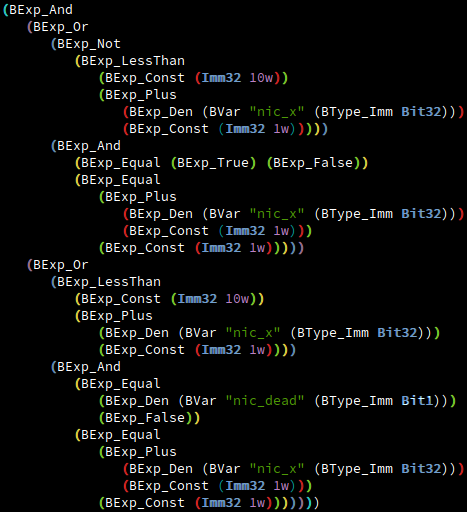
\includegraphics[scale=.65]{figures/proof_wp_exp.png}
	\centering
	\caption{Autogenerated weakest precondition for proof of Theorem \ref{proof_ht_thm}.}
	\label{proof_wp_exp}
\end{figure}

Then, the proof consist of consecutively rewriting following the definition of $bir\_eval\_exp$ and the definition it uses until the goal only contains $$bir\_env\_read~(BVar~``nic\_x"~(BType\_Imm~Bit32))~bir\_state.bst\_environ$$ and similarly for $nic.dead$. Let's call those expressions $x\_val$ and $dead\_val$ respectively. For expressions, BIR semantic is defined over immutable and constant values. Therefore, we need to establish an equivalence between the values that we currently have.

\begin{lemma}
	\begin{equation*}
		\exists x\_imm.~x\_val = BVal\_Imm~x\_imm
	\end{equation*}
	\label{proof_exists_x_imm}
\end{lemma}
\begin{proof}
Assuming well-typedness and initialization, this theorem immediately results from the BIR semantic.
\end{proof}

\begin{lemma}
	\begin{equation*}
		\exists x\_word.~x\_imm = Imm32~x\_word
	\end{equation*}
	\label{proof_exists_x_word}
\end{lemma}
\begin{proof}
This lemma is part of the BIR semantic, as one of the six conjuncts of the \texttt{bir\_imm\_t\_nchotomy} theorem, which establishes this existence theorem for every BIR immutable types.
\end{proof}

Now, using Lemma \ref{proof_exists_x_imm}, we are able to substitute all occurrences of $x\_val$ into $BVal\_Imm~(Imm32~x\_word)$, and similarly for $dead\_val$. Finally, rewriting the goal using the full set of BIR semantic theorems and some rewriting rules, the goal reduces to an expression free of BIR terms:

\begin{equation} \label{proof_wp_word_goal}
\begin{split}
&(dead\_w = 0w) \land (x\_w = 0w) \implies\\
&\Big(\neg(10w <_{+} x\_w + 1w) \lor \big((1w = 0w) \land (x\_w + 1w = 1w)\big)\Big)~\land\\
&\Big((10w <_{+} x\_w + 1w) \lor \big((dead\_w = 0w) \land (x\_w + 1w = 1w)\big)\Big)
\end{split}
\end{equation}

An {SMT} solver is able to prove this goal. Interestingly, HOL4 simplification procedures are also able to prove it. However, they won't be able to prove it for more complicated ones or will be less effective than SMT solvers.
\end{proof} % End of Hoare Triple proof

Finally, using the deduction rule with Theorems \ref{proof_R_inj_thm}, \ref{proof_b_thm}, \ref{proof_R_def}, \ref{proof_ht_thm}, \ref{proof_eq_thm} and \ref{proof_d_thm}, in that order, concludes this proof.
\renewcommand\qedsymbol{$\blacksquare$}
\end{proof}













































\end{multicols}

\printbibliography

\newpage
\section*{Appendix. {\normalsize\textit{Figures}}}
\renewcommand{\thefigure}{A.\arabic{figure}}
\setcounter{figure}{0}

\begin{figure}[htbp]
	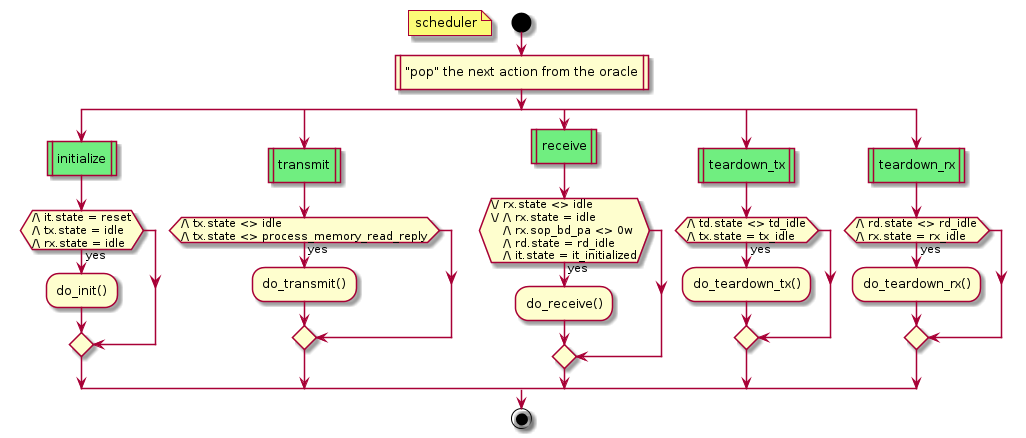
\includegraphics[width=\columnwidth]{figures/flowchart-scheduler.png}
	\centering
	\caption{Flowchart of the scheduler of the NIC model. Green nodes represent condition statements, here they represent the value of the popped action from the oracle. The full dot represents the entry point, and the other point the exit point.}
	\label{flowchart-scheduler}
\end{figure}

\begin{figure}[htbp]
	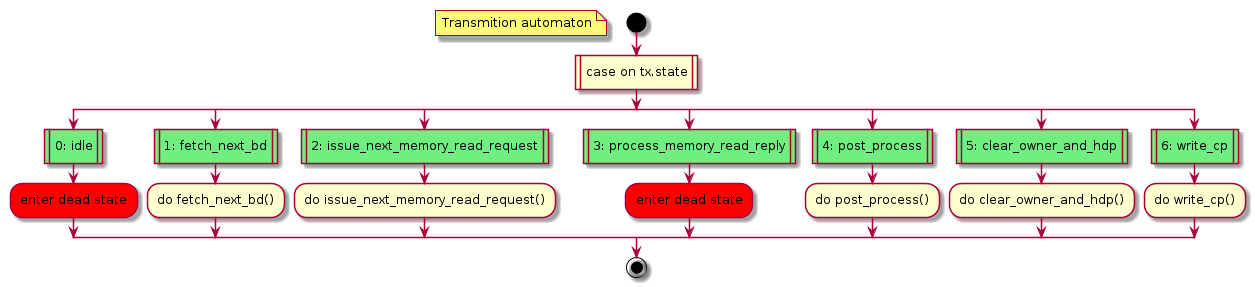
\includegraphics[width=\columnwidth]{figures/flowchart-tx.png}
	\centering
	\caption{Flowchart of the transmission automaton of the NIC model. Green nodes are similar to the ones of Figure \ref{flowchart-scheduler}. Red nodes represent non autonomous transitions leading to dead states.}
	\label{flowchart-tx}
\end{figure}

\begin{figure}[htbp]
	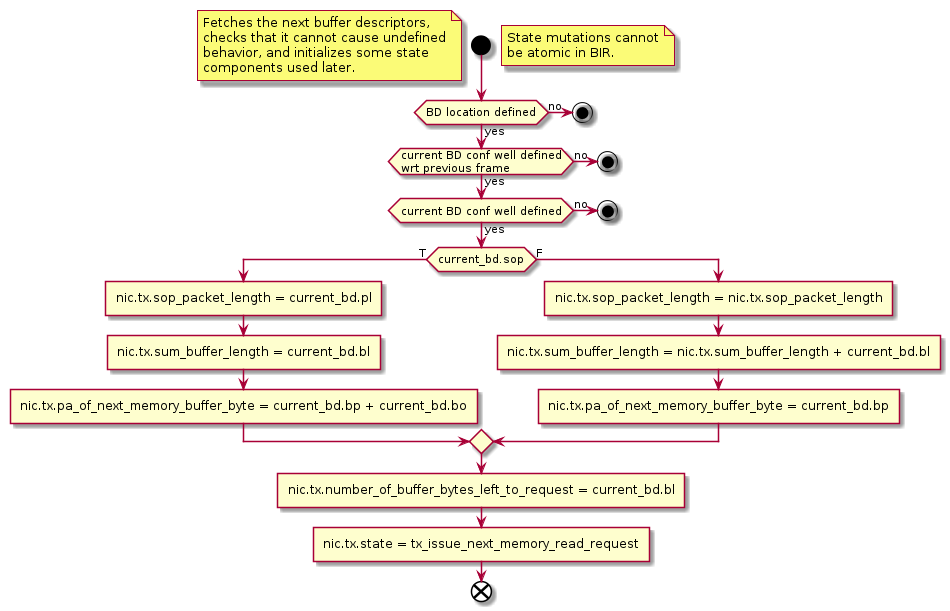
\includegraphics[width=\columnwidth]{figures/flowchart-tx_fetch_next_bd.png}
	\centering
	\caption{Flowchart of the \texttt{fetch\_next\_bd} transition of the transmission automaton of the NIC model. The full dot represent the entry point, $\bigotimes$ represents the exit point and the other dots are shorthands to represent dead transitions (the symbols have been changed because of technical limitations of the tool used to draw the diagram).}
	\label{flowchart-tx_fetch_next_bd}
\end{figure}

\end{document}























